\subsection{IGS Ludhiana Website}
{\bf Introduction to IGS Ludhiana}\\
IGS stands for Indian Geotechnical Society which is a great society whose aim is to promote cooperation amongst engineers and scientists for the advancement and dissemination of knowledge in the fields of Soil Mechanics, Foundation Engineering, Soil Dynamics, Engineering Geology, Rock Mechanics, Snow and Ice Mechanics and any allied fields related to Geotechnical Engineering and their practical applications. Indian Geotechnical Society, New Delhi (IGS) has opened its 35th Chapter in Ludhiana with an aim to address the local problems faced by the people of Punjab in general and civil engineering community in particular. It will provide a platform to the engineers, scientists, industrialists and others who are actively associated with the geotechnical works to come together to interact, collect, synthesize and collate valuable information on geotechnical engineering aspect of Civil Engineering for betterment of the community.\\\\
Our college got a chance to make a website for this. Inauguration of this website was also in our college. It was a great achievement for our college.\\\\
Along with me this task was given to four more students: Jaspreet Kaur, Navdeep Bagga, Damanpreet Singh and  Vigasdeep. We divided all the work so that we make this website up in a short period (two days). The Website is developed in Wordpress, an Open Source Web Framework. Different works were given to each student. The website can be found at :\\\\
http://gndec.ac.in/~igs/ldh/ \\\\
Selected the theme: Twenty eleven [A ver stable theme and easy to configure]\\
Plugin Installed : News announcement scroll [This plugin create a vertical scroll news or Announcement for your wordpress site, we can embed this in sidebar, Multi language support.}\\\\
{\bf My Contribution}\\
Tweaked CSS \& Header Files. \\
Handled all the graphics of the website. Made the banner of the Website in Gimp.\\
\newpage
\begin{figure}[h]
\centering 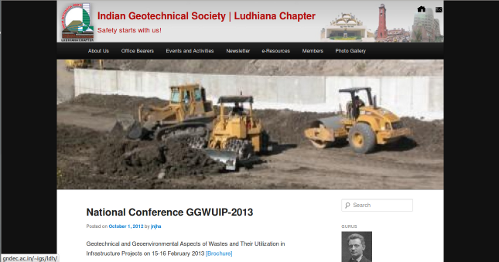
\includegraphics[scale=1.0]{igs.png}
\caption{IGS Website}
\end{figure}
 
{\bf TECHNOLOGIES USED}\\\\
{\bf Wordpress}\\
WordPress is a free and open source blogging tool and a content management system (CMS) based on PHP and MySQL. It has many features including a plug-in architecture and a template system. WordPress is used by over 16.7\% of all new websites. WordPress is currently the most popular blogging system in use on the Web.\\\\
Its Features are :\\
\begin{itemize}
\item Themes : WordPress users may install and switch between themes. Themes allow users to change the look and functionality of a WordPress website or installation without altering the information content or structure. 
\item Plugins : One very popular feature of WordPress is its rich plugin architecture which allows users and developers to extend its abilities beyond the features that are part of the base install.
\item Widgets : Widgets are small modules that offer users drag-and-drop sidebar content placement and implementation of many plugins' extended abilities. Widgets allow WordPress developers to add functionality to their sites.
\item Multi-user and multi-blogging
\end{itemize}
\newpage
\begin{figure}[h]
\centering 
\includegraphics[scale=0.2]{word.png}
\caption{Wordpress}
\end{figure}
{\bf GIMP}\\\\
GIMP (GNU Image Manipulation Program) is an image retouching and editing tool and is released under the GPLv3 license as free and open-source software. There are versions of GIMP tailored for most operating systems including Microsoft Windows, Mac OS X and Linux.\\\\
GIMP has tools used for image retouching and editing, free-form drawing, resizing, cropping, photo-montages, converting between different image formats, and more specialised tasks. Animated images such as GIF and MPEG files can be created using an animation plugin.
\begin{figure}[h]
\centering 
\includegraphics[scale=0.4]{gimp.png}
\caption{Wordpress}
\end{figure}
\newpage

\subsection{Operating UDF Disks}
{\bf Introduction to UDF}\\
Universal Disk Format (UDF) is a profile of the specification known as ISO/IEC 13346 and ECMA-167 and is an open vendor-neutral file system for computer data storage for a broad range of media. In practice, it has been most widely used for DVDs and newer optical disc formats, supplanting ISO 9660. Due to its design, it is very well suited for incremental updates on both recordable or (re)writable optical media. UDF is developed and maintained by the Optical Storage Technology Association (OSTA).\\\\
{\bf Different between UDF and ISO Disks}\\\\
The ISO File System ISO is the original method, and the one used in “pressed” CD-ROMs, such as the Windows XP CD-ROM. In this system, all the files to be written are selected, and then written to the disc as continuous tracks, together with a Table of Contents (TOC) which defines where the data of a file is to be found in the track. Together, these files and TOC form a session. If the disc has not been filled, it can be put back into the writer, and a further session written. The TOC for the new session will link back to the previous TOC, so that all the files on the disc appear as being on a single CD.\\
Because of this method of writing, the files cannot be individually changed or deleted. If on a CD-RW disc, they can only be erased as a whole. The ISO file system is mostly used, therefore, with CD-R media.\\
Every session has an overhead of about 14 MB, so this is a very wasteful method if used to write files individually rather than in batches.\\
The resulting burned disc can be read in any PC CD-ROM drive (except, perhaps, some very obsolete ones) using only the normal software of any version of Windows. \\\\
The UDF File System is a quite different approach, in which a CD-RW disc is first formatted into packets which then behave very much like the sectors of a hard disc. While the file system can be used in discs organised in tracks, as with the ISO system, and is also used on DVD discs, the term “UDF” will be used here in the sense of it using this packet writing base on CD-RW discs. Files can be written to a series of packets as an individual operation, and, later, those of a file can be selectively erased or updated. Therefore, such a CD is described as behaving as a “giant floppy” (or very slow, small hard disc). When UDF is implemented, files can be dragged and dropped to and from the CD in Windows Explorer, just as to and from a hard disc; or, to give another example, the CD can be selected as the drive to use in a “Save As” dialog in a program. The UDF file system was often used in earlier versions of Windows through third party packages such as Direct CD.\\
Reading such discs needs special software in earlier versions of Windows, and may not be possible with all CD drives, even when that software is present.\\
While there is a variant of the UDF method that can be used to write to CD-R media, it is rarely used. Thus when using UDF DVDs, one can come accross problem where either it does not mount in the system or if get mounted shows empty disks. I came accross one such situation, where I had following experience.\\\\
{\bf My Experience with UDF Disk}\\\\
After getting the DVD, first of all I tried to mount it on ubuntu. After creating a lot of sounds, it popped out a message ``could not mount due wrong fs type, bad option, bad superblock". Even manual mount through command line, did not helped. After searching for the error, I found that there is a command for installing udf library or something. It solved someone's problem on stackflow, but even that was not useful for me. Some links said that this error is not usual, as of most the DVDs are udf format and they are easily mounted in ubuntu. So problem might be with the software in which they were burned. The solution for this: a patch for the kernel(limited on versions like 2.6 etc) is available, apply it, compile it, this may help. I was pretty doubtful on this solution as I am running the latest kernel.\\\\
Then I moved on to windows. I have windows 7. There, upon mounting the drive, I could just see that CD was almost full, but on opening it appeared to be blank. I searched for some UDF reader in windows. I found IsoBuster software. Downloaded trial version. With this I could
detect that something was within the CD. I could neither extract it, as that required getting the paid version (I hate windows for this
only. when you start knowing about something, it flashes back ``GET PAID VERSION" :-X) nor I could copy them. Then I installed some other
CD burner softwares like Nero, adptec udf reader, but to no avail. Upon searching I found, those suffering from this problem can run
these type of CD's on window xp. I tried even on that. That was even worse. Windows showed a CD with 63 (or something) Mb and totally
empty. So our case appeared to be totally different. Then I found that CD can found empty even when it is corrupted. So then I searched for
CD recovery tool in window. Found one and then I was even able to recover data and then I got to know that in trial version, I can
recover only 1 GB data. Somehow I managed to recover all the data. \\\\
Thus from all this experience I get accross a conclusion :
\begin{itemize}
\item Never use a third party Software to burn the CD or DVD.
\item Don't burn the DVD as UDF unless you want a large data to be burned.
\item Always chech whether the CD or DVD burned is compatible with all the platforms.
\end{itemize}


 
